\documentclass[a4paper,fleqn,usenatbib,useAMS]{mnras}

%\usepackage[draft]{graphicx}  % this stop figures from rendering
\usepackage{graphicx}	% Including figure files
\usepackage{amsmath}	% Advanced maths commands
\usepackage{amssymb}	% Extra maths symbols
\usepackage{multicol}        % Multi-column entries in tables
\usepackage{bm}		% Bold maths symbols, including upright Greek
\usepackage{pdflscape}	% Landscape pages
\usepackage{IEEEtrantools} % for stacked equations

\newcommand{\numax}{\ensuremath{\nu_{\textrm{max}}}}
\newcommand{\dnu}{\ensuremath{\Delta\nu}}
\newcommand{\teff}{\ensuremath{T_{\textrm{eff}}\:}} 
\newcommand{\kep}{\ensuremath{Kepler}\:}
\newcommand{\pdet}{\ensuremath{P_{\rm det}\:}}
\newcommand{\kp}{\ensuremath{K_{p}\:}}
\newcommand{\tobs}{\ensuremath{T_{\textrm{obs}}\:}} 
\newcommand{\imag}{\ensuremath{I_{\textrm{mag}}\:}} 
\newcommand{\msol}{\ensuremath{M_{\odot}\:}} 
\newcommand{\logg}{\ensuremath{{\rm log}(g)\:}} 


\newcommand{\bibtex}{\textsc{Bib}\!\TeX} % bibtex. Not quite the correct typesetting, but close enough

\usepackage[T1]{fontenc}
\usepackage{ae,aecompl}
%\usepackage{newtxtext,newtxmath}  % new version
\usepackage{txfonts}  % old version

\title[Asteroseismology with Machine Learning]{TESS Asteroseismic Predictions for Red Giants using Machine Learning}

\author[M. Schofield et al.]{M. Schofield$^{1, 2}$\thanks{E-mail: mxs191@bham.ac.uk}, G. R. Davies$^{1, 2}$, W. J. Chaplin$^{1, 2}$, A. Miglio$^{1, 2}$
\\
% List of institutions
$^{1}$Department of Physics and Astronomy, the University of Birmingham, Birmingham B15 2TT, UK \\
$^{2}$Stellar Astrophysics Centre (SAC), Department of Physics and Astronomy, Aarhus University, Ny Munkegade 120, DK-8000 Aarhus C, Denmark}


%\thanks{Contact e-mail: \href{mailto:mxs191@bham.ac.uk}{mxs191@bham.ac.uk}}\thanks{Present address: Department of Physics and Astronomy, the University of Birmingham, Birmingham B15 2TT, UK}



\date{Last updated 2017 May 31; in original form 2017 May 31}
\pubyear{2018}

\begin{document}
\label{firstpage}
\pagerange{\pageref{firstpage}--\pageref{lastpage}}
\maketitle

\begin{abstract}
For the first time. a classifier was used as a way to select solar-like asteroseismic targets before a future mission. The classifier managed to identify the detectable solar-like oscillations inside \kep Red Giants with a 0.98\% precision. To do this, it used only the global parameters \texttt{[log($g$), $\pi$, \teff, [M/H], \imag]}.

The same classifier was also used on the \kep stars after they had been degraded into TESS-like observations. The classifier scored 0.90\% and 0.81\% when made to look like 1-year and 27-days of TESS-like data, respectively. This classifier could be used to select asteroseismic targets for TESS in the Continuous Viewing Zone \citep{ricker_transiting_2014}, and as a way of investigating any target selection bias in previous missions such as K2 and CoRoT.
\end{abstract}



\section{Introduction}

\begin{itemize}
\item We use a classifier to make detectability predictions for TESS \citep{ricker_transiting_2014}
\item Mention the application to PLATO \citep{rauer_plato_2014}.
\item Supervised classifiers have been used to determine the evolutionary state of variable stars: \citet{debosscher_automated_2007}, \citet{sarro_automated_2009}, \citet{nun_supervised_2014}, \citet{elorrieta_machine_2016}. Similarly, unsupervised classifiers \citep{valenzuela_unsupervised_2018} and regression \citep{ness_cannon_2015} have also been used to determine evolutionary stages.
\item A neural network has also been used to identify the evolutionary stage of Red Giant stars (\citet{hon_deep_2017}, \citet{hon_deep_2018}).
\item Machine learning has also been used to calculate stellar parameters \citep{bellinger_fundamental_2016}, including oscillation frequencies \citep{davies_oscillation_2016}.
\item One reason to use Machine Learning for target selection is that it can reverse-engineer target selection bias, for example in K2 \citep{lund_K2P2_2015} and CoRoT \citep{baglin_corot:_2006}. This can provide insights into the formation history of the galaxy: \citet{thomas_galactic_2017}.
\item Summarise the Chapters.
\end{itemize}


\iffalse
Satellites such as $Kepler$ have allowed asteroseismology of solar-like and Red Giant stars to advance rapidly since the last century \citet{chaplin_asteroseismology_2013}. Power spectra can now be resolved to detect individual modes of oscillation in Main Sequence and Red Giant stars (\citet{lund_standing_2017}, \citet{davies_asteroseismology_2016}).

Future space missions such as TESS \citep{ricker_transiting_2014} and PLATO \citep{rauer_plato_2014} will add to our understanding of stellar structure and evolution. These missions will provide a large amount of high-precision data. More than ever, the field of stellar astrophysics will require tools to perform big-data analysis. %\citep{kremer_big_2017}. 

One of the tools than can be used to handle the large amount of data from future missions is Machine Learning. In this work, Machine Learning was used to create a TESS target selection function using the set of $Kepler$ Red Giant Branch, Red Clump and Secondary Clump stars from Davies et al. (in prep). This algorithm is publicly-available\footnote{https://github.com/MathewSchofield/TRG}. It can be downloaded and used as a target selection function for any future space mission.

In most situations, Machine Learning is used to solve problems in one of two ways: either by using Supervised or Unsupervised Learning. Unsupervised Learning involves problems where there are no known labels or results. Conversely, Supervised Learning involves problems where there is a known result.

In Unsupervised Learning, there are no known results/labels. The aim of Machine Learning in this case would be to find trends between variables. This has been be used to identify the evolutionary stage of stars by analysing their lightcurves without using previously labelled data. The evolutionary stage of variable stars has been determined in this way using an Unsupervised classifier \citep{valenzuela_unsupervised_2018}. Similarly, a neural network has been used to identify the evolutionary stage of Red Giant stars (\citet{hon_deep_2017}, \citet{hon_deep_2018}).

Supervised Learning has also been used to classify the evolutionary stage of variable stars (\citet{nun_supervised_2014}, \citet{elorrieta_machine_2016}). In these papers, classifying evolutionary stage was treated as a Supervised problem because previously labelled data were used. This previously labelled data is known as training data: this is used to train the Machine Learning algorithm. In the problem of variable stars, lightcurves that had already been classified were used to train the algorithm (this is the training dataset). This algorithm was then used to classify the lightcurves of unidentified stars (this is known as the testing dataset). In this way, the authors were able to identify the evolutionary stage of every star in their sample.

In this work, a classifier was \textit{not} used to identify the evolutionary stage of stars. For the first time, a supervised classifier was used here to identify which solar-like modes could be detected in Red Giant stars with TESS. These modes were given to the classifier as known labels, so this is a Supervised Learning problem\footnote{https://machinelearningmastery.com}.

A classifier was used here to identify which solar-like modes could be detected inside Red Giant stars with TESS. As a result, this algorithm can be used as the target selection function for TESS. Furthermore, this code has been written specifically for easy adaption to other satellites. It can therefore also be used as the target selection function for K2, CoRoT and PLATO.

%The aim of this work is to use Machine Learning to make predictions about mode detectability (\pdet) in Red Giant stars. In this case, \pdet is a known label, so this is a Supervised Learning problem\footnote{https://machinelearningmastery.com}.

Within Supervised Learning, two common algorithms that are used are Classification and Regression. In Regression, the relationship between variables is interpreted using a measure of uncertainty (such as using $\chi^{2}$ tests). Models are fitted using the independent data, and uncertainty is measured. The models are then improved by reducing this uncertainty. Note that regression is used when the label is continuous. For example, predicting the magnitude of a star is a problem suited to regression, as a star can have any magnitude \citep{steinhardt_nonparametric_2018}.

Conversely, Classification algorithms work by assessing similarity\footnote{http://www.simafore.com}. In Classification, the training set is separated into groups based on the similarity of the data. The more information that was gained by splitting the data, the better. %For example, if the problem were to separate Red Giant stars from Main-Sequence stars, a star could be classified as either a Red Giant (1), or not a Red Giant (0). In this example, having a Luminosity above $\sim10L_{\odot}$ would be a strong indicator that the star was a Red Giant so the data could be separated into groups here. The classifier would continue to separate the dataset until the Red Giant and Main Sequence samples were distinct. 
Examples of classifiers being used to identify the evolutionary stages of stars can be found in \citet{ness_cannon_2015} and \citet{wu_mass_2017}.

In this work, a classifier was not used to identify the evolutionary stage of stars. Instead, it was used to identify which solar-like modes could be detected by TESS, and which could not. Individual fitted modes from Davies et al. (in prep) were degraded to look like TESS observations. The detectable solar-like modes from this degraded set were then identified by a classifier. By separating the stars into those with detected modes and those without, a classifier was used to select the optimal targets for TESS to observe.

Firstly, Section \ref{sect: dataset} describes how the size of the datasets were increased to improve the predictive ability of the classifier. Section \ref{sect: tess-like} then outlines how the timeseries of every star were treated before transforming them into power spectra. Section \ref{sect: det_test} goes on to explain the detection test that was run on the solar-like oscillations. This returned a probability of detection \pdet for every mode. Each mode was grouped into a discrete class depending upon its detection probability; each mode was either very likely to be observed (0.9-1.0, class '2'), quite likely (0.5-0.9, class '1'), or unlikely (0.0-0.5, class '0').

Lastly, Section \ref{sect: classifier} illustrates how the stars were classified. The stars were put into a group with detected modes, and a group without. This was done by giving a supervised classifier photometric and spectroscopic information on every target from APOKASC \citep{pinsonneault_apokasc_2014}. 70\% of the stars were used to train the classifier; 30\% of the sample was kept to test the algorithm. The classifier was given global asteroseismic and spectroscopic information, as well as mode detection probabilities of the stars in the training set. It then made predictions about mode detectability on the testing set.

The classifier recognised patterns between the variables in the training set, and successfully made predictions about mode detectability with a 0.98\% precision for the original \kep data. It achieved a precision of 0.90 for 1 year of TESS-like observation, and 0.81 for 27 days of TESS-like observation.
\fi


\section{The dataset}
\label{sect: dataset}

The data to perform Machine Learning on are the 1000 \kep Red Giants from Davies et al. (in prep). These are shown in Figure \ref{fig:dataset}.
\begin{figure}
	\centering
	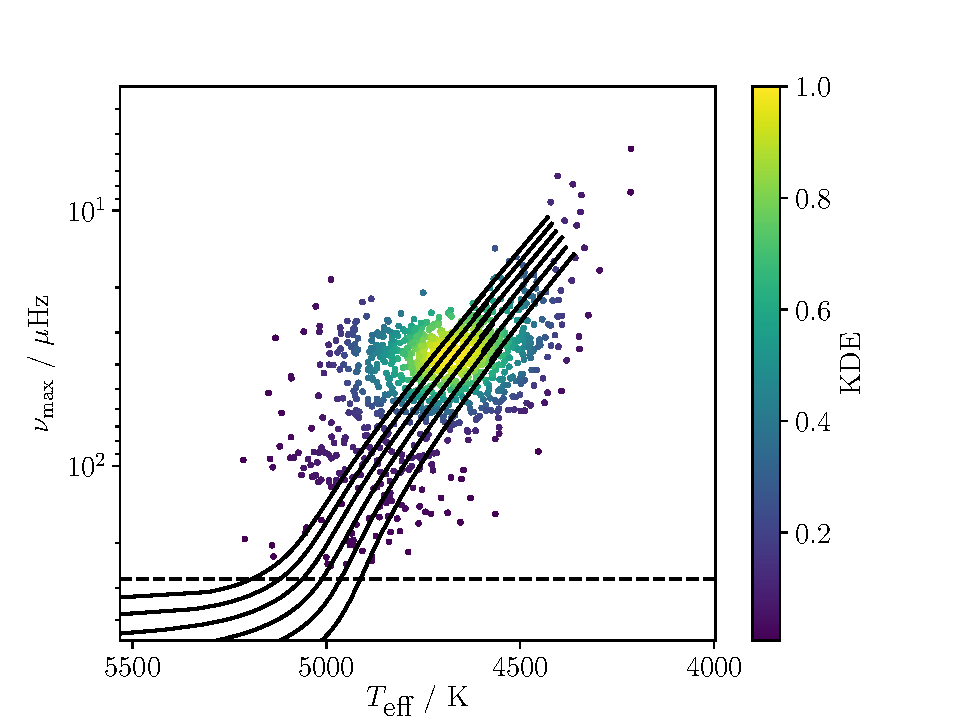
\includegraphics[scale=0.5]{Plot1_HR.pdf}
	\caption{The 1000 \kep Red Giants from Davies et al. (in prep). The colourbar shows the relative density of points with Kernel Density Estimation. The evolutionary tracks range from 0.9-1.5\msol.}	
	\label{fig:dataset}
\end{figure}
The radial and quadrapole modes of these stars have been fitted by Davies et al. (in prep). The frequency, height, width and background of each mode in the 1000 stars had been individually fitted. The spectroscopic parameters of these stars (\teff, \logg, [M/H]) were available from APOKASC \citet{pinsonneault_apokasc_2014}. The apparent magnitudes are from the $Tycho$-2 catalogue \citet{hog_tycho-2_2000}. Lastly, the parallaxes are from $Gaia DR2$ \citet{lindegren_gaia_2018}.

Machine Learning performs best when a large dataset is available to train the algorithm on. In order to increase the size of the dataset above 1000, the magnitude of each \kep star was perturbed. Each star had its apparent magnitude perturbed 100 times. 

The instrumental (shot) noise models of \kep and TESS were used as PDFs to draw apparent magnitudes from. These were used because they provide realistic distributions of the number of stars at different magnitudes that the satellites observed/will observe. Many more fainter stars are observed than brighter stars because the volume of space that contains stars increases as the distance of observation increases.

The shot noise model of $Kepler$ depends on the $Kepler$ magnitude of the star, $K_{p}$. This noise model is from \citet{gilliland_initial_2010}. The \texttt{RMS} noise, $\sigma$, is given by
\begin{equation}
\sigma = \frac{10^{6}}{c} \times \sqrt{c+9.5 \times 10^{5}\Bigg(\frac{14}{K_{p}}\Bigg)^{5}}  {\rm ppm},
\label{eq:kep noise}
\end{equation}
where $c$ is the number of detected electrons per cadence. It is given by
\begin{equation}
c = 1.28 \times 10^{0.4(12-K_{p})+7} .
\end{equation}

The equivalent TESS shot noise model was taken from \citet{sullivan_transiting_2015}. The \texttt{RMS} noise was calculated using photon counting noise, the noise from background stars, the readout noise and the systematic noise. These four noise sources were then summed in quadrature to give the total TESS noise.

\iffalse
which depends on the $I_{c}-$band magnitude of the star and the number of pixels in the photometric aperture used when observing the star. This is given by
\begin{equation}
N_{\rm aper} = 10 \times (n+10) , 
\end{equation}
where $n$ is
\begin{equation}
\label{eq:tess noise}
n = 10^{-5.0} \times 10^{ 0.4 \times (20-I_{\rm mag})} .
\end{equation}
\fi

The \kep and TESS noise models were used as the PDFs to draw stellar magnitudes from. 100 magnitudes were drawn for every \kep Red Giant. After removing gaps in the data, this left 60,000 samples. The lightcurves of this much larger \kep dataset were then degraded to look like TESS observations.



\section{Imputing Imag values}
\label{sect: impute}

741 of the 1000 \kep stars have measured \imag values from $Tycho-2$ \citep{hog_tycho-2_2000}. \imag is needed for every star to calculate the TESS shot noise level. In order to keep the remaining stars in the dataset, the \imag values were imputed.

\imag values for the missing stars were imputed using random forest regression. Like a random forest classifier, random forest regression is another example of supervised learning: in both cases there is a known label to predict (here the label is \imag). Supervised learning involves separating the data into training and testing datasets. In classification, the data is grouped by similarity. In regression, the difference between the regression model and 'true' values is evaluated, and iteratively reduced. This difference is evaluated using the Sum of Squared Errors (SSE);
\begin{equation}
{\rm SSE} = \sum_{i=1}^{N} (x_{i} - \bar{x})^{2}.
\end{equation}

Random forest regression was used in this way to get the missing \imag values. This could have been done using only the 741 available \imag values of the 1000 stars. However, in order to improve the predictions made from the regression, a selection of the brighter stars in the $Kepler$ Input Catalogue (KIC; \citet{brown_kepler_2011}) were used alongside the 741 fitted Red Giants. In total, 2366 stars were used to train and test the regression.

The KIC provides a variety of magnitudes, but not the 2MASS\footnote{https://www.ipac.caltech.edu/2mass/} \imag. \imag was calculated for the KIC stars using the 2MASS magnitudes $J_{\rm mag}, H_{\rm mag}, K_{\rm mag}$, and the SDSS \citep{kollmeier_sdss-v:_2017} magnitude $i_{\rm mag}$. Not all of these magnitudes were available for the 259 fitted $Kepler$ stars from Davies et al. (in prep).

Firstly, an equation from \citet{bilir_transformations_2008} was used to calculate $(R-I)$;
\begin{equation}
(R-I) = c_{1}(J-H) +c_{2}(H-K) + c_{3} .
\end{equation}
The coefficients $c_{1}, c_{2}$ and $c_{3}$ vary with metallicity and are given in the paper. Secondly, $(i-I)$ was calculated from $(R-I)$ using an equation from \citet{jordi_empirical_2006};
\begin{equation}
\label{eq: i-I}
(i-I) = 0.247(R-I) + 0.329 .
\end{equation}
It is then straightforward to calculate \imag for every KIC star,
\begin{equation}
\imag = -(i-I) + i_{\rm mag} .
\end{equation}

Once \imag values were calculated for every KIC star in the dataset, they were used in random forest regression along with [\kp, [M/H], \teff] to predict \imag value for the 259 $Kepler$ stars.

70\% of the dataset was used to train the algorithm; 30\% was used to test it's accuracy. The results of the random forest regression are shown in Figures \ref{fig:imag test hist} and \ref{fig:imag test scatter}. Figure \ref{fig:imag test hist} shows that the distribution of predicted value matches the 'true' \imag values closely. Figure \ref{fig:imag test scatter} shows that there is no offset between the predicted and 'true' values; the mean difference between the two is -0.01 mag. Furthermore, the standard deviation of the difference is only 0.27 mag, and the regression achieves an accuracy of 0.90. To summarise this, random forest regression predicts the \imag values in the test dataset well.

After testing the regression, the algorithm was used to make predictions on the $Kepler$ stars without known \imag values. The distribution of predicted values is shown in Figure \ref{fig:imag train}, along with the entire KIC sample used to train the regression in blue for comparison.
\begin{figure}
	\centering
	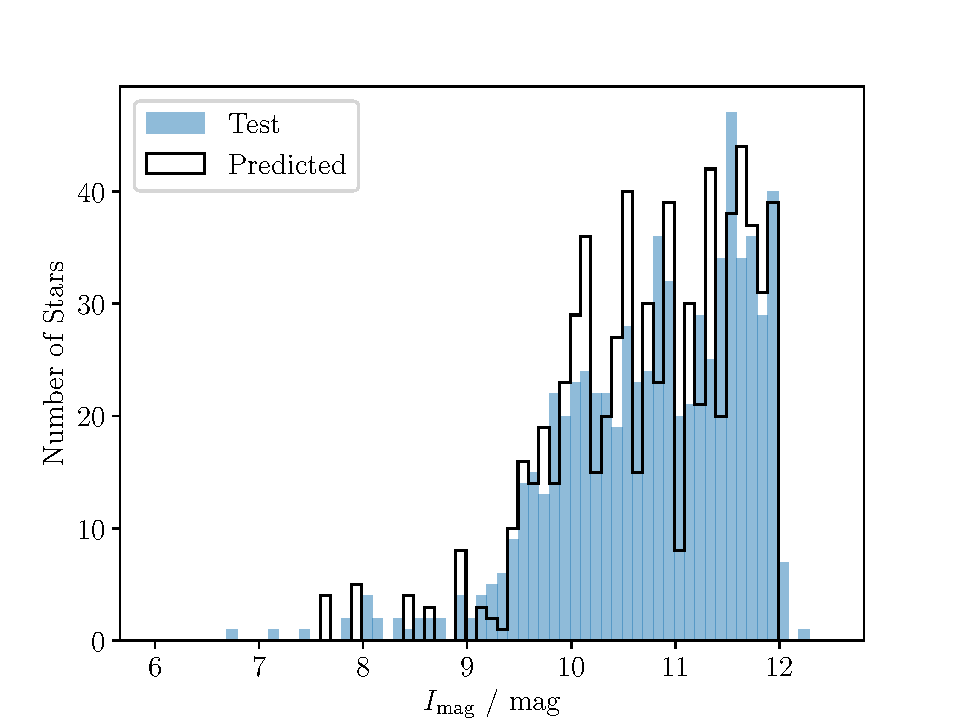
\includegraphics[scale=0.5]{Plot3_Imag_tested_distribution_50kstars}
	\caption{The \imag distribution of the KIC stars used to test the random forest regression. The 'true' values used to test the algorithm are shown in blue. The black histogram shows the distribution of values that the random forest regression predicted for that dataset.}	
	\label{fig:imag test hist}
\end{figure}
\begin{figure}
	\centering
	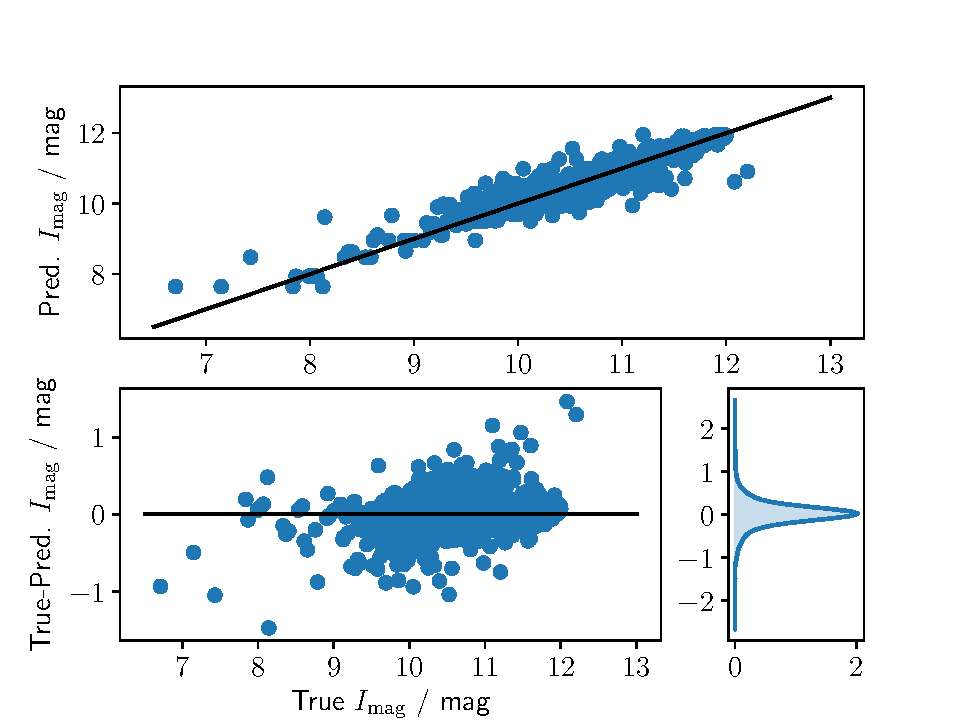
\includegraphics[scale=0.5]{Plot4_Imag_scatter_50kstars}
	\caption{The true \imag values of the KIC stars use to test the algorithm, compared to their predicted values. The mean difference between the two sets of values is -0.01 mag, with a standard deviation of just 0.27 mag.}	
	\label{fig:imag test scatter}
\end{figure}
\begin{figure}
	\centering
	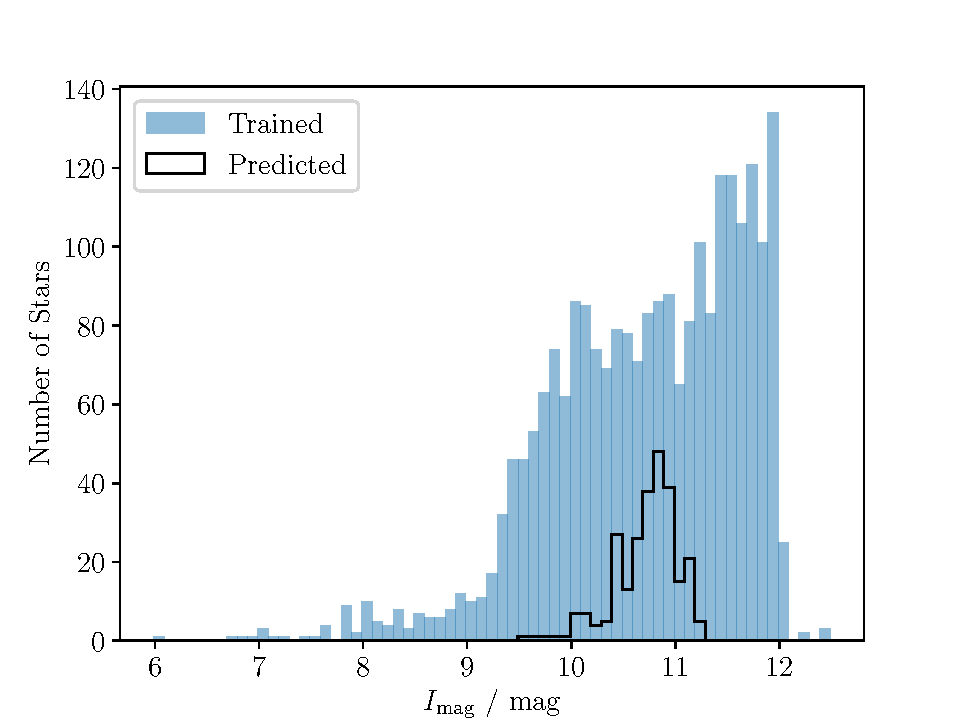
\includegraphics[scale=0.5]{Plot3_Imag_trained_distribution_50kstars}
	\caption{The \imag distribution of the KIC stars used to train the random forest regression is shown in blue. The predicted values for the stars without $I$-band magnitudes is shown in black.}	
	\label{fig:imag train}
\end{figure}



\section{Modifying Kepler data to look like TESS}
\label{sect: tess-like}

Before a classifier could be used on the Red Giant sample, the timeseries data from \kep needed to be modified for TESS. These adjustments were made in the time domain before the signal was converted to the frequency domain.

Several different adjustments needed to be made to the \kep \ data. One difference between the missions is the length of observation. The \kep \ mission observed stars for up to 4 years. TESS' nominal 2 year mission will observe stars for between 27 days to 1 year, according to the ecliptic latitude of the stars \citep{ricker_transiting_2014}.

\iffalse
\begin{figure}
	\centering
	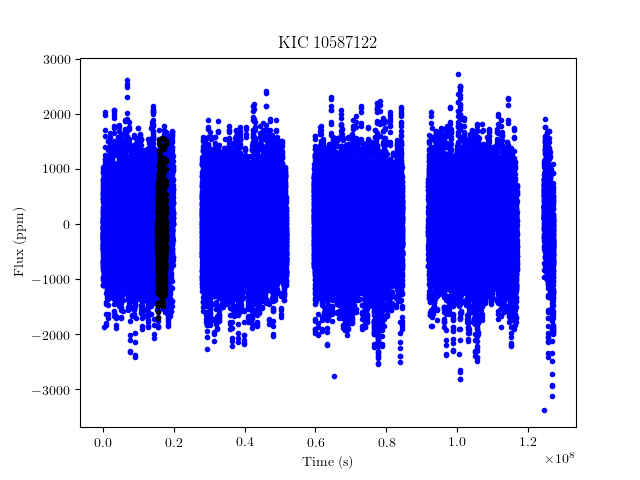
\includegraphics[scale=0.6]{timeseries_10587122}
	\caption{The 4-year long Power Spectra of KIC 10587122 is plotted in blue. Overplotted is the 27-day time segment with most coverage (the period with fewest gaps in the data). Reducing the length of observation this drastically will badly hamper mode detectability.}	
	\label{fig:ts plot}
\end{figure} 
\fi

As well as reducing the dataset length, the bandpass of observation needed to be adjusted. TESS will observe in a much redder bandpass than that of \kep. This has the effect of reducing the amplitude of stellar signals (i.e the signals due to stellar granulation and solar-like oscillations) \citep{ballot_visibilities_2011}. \citet{campante_asteroseismic_2016} found this bandpass correction in the amplitude spectrum to be 0.85 for TESS.

\iffalse
\begin{figure}
	\centering
	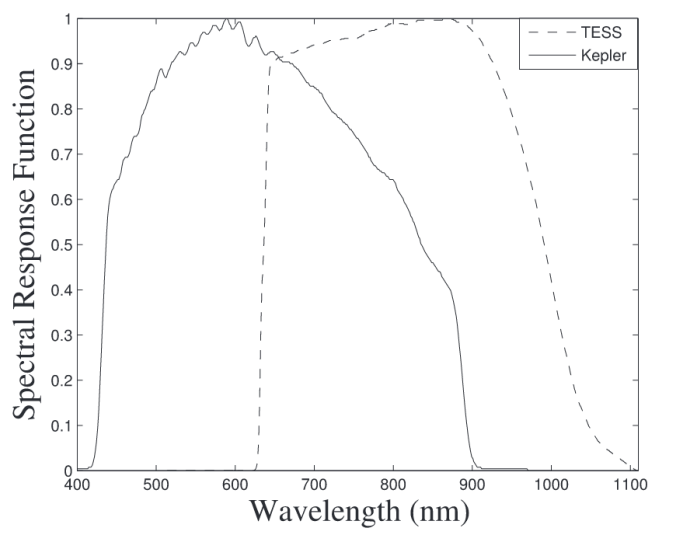
\includegraphics[scale=0.4]{bandpass.png}
	\caption{The bandpass' of the $Kepler$ and TESS missions. TESS will observe at longer (i.e redder) wavelengths than $Kepler$. This will reduce the amplitude of oscillations and granulation, whilst the white noise level will by unaffected. Image taken from \citet{placek_combining_2016}.}	
	\label{bandpass}
\end{figure} 
\fi

Thirdly, the noise level for a given star in \kep \ is lower than the noise level in TESS. %The noise level for the \kep \ satellite depends on the \kep \ magnitude of the star, equation \ref{eq:kep noise}. 
Noise from TESS was calculated for each star and added to the timeseries (see Section \ref{sect: dataset}).

These three adjustments - the length of observation, the bandpass, and the noise level (see Section \ref{sect: dataset}) - were performed in the time domain. From the original \kep timeseries, these adjustments were made:
\begin{enumerate}
\item Apply a 4-$\sigma$ clip to the dataset to remove spurious points.
\item Cut the 4 years of data down to the reduced dataset length (27 days to 1 year). Use the 27 days to 1 year of data with the fewest gaps.%, see Figure \ref{fig:ts plot}.
\item Adjust the bandpass by multiplying the flux by 0.85.
\item Add TESS instrumental noise to the timeseries. To do this, calculate the TESS \texttt{RMS} noise level (Section \ref{sect: dataset}). For each flux value in the timeseries, draw a random number from the normal distribution. Multiply the \texttt{RMS} noise by each flux value. Add this to the original flux values in the timeseries.
\item Use the Lomb-Scargle periodogram to convert the signal from the time to frequency domain.
\end{enumerate}

Examples of the TESS-like power spectra are shown in Figures \ref{Power Spectra} and \ref{overplotted PS}. Power spectra were generated for the original 4-year \kep sample, 1 year of TESS observations and 27 days of TESS observations. Once the timeseries had been made to look like TESS observations, a detection test was then run on the radial modes of every star in these 3 datasets. 

\begin{figure}
	\centering
	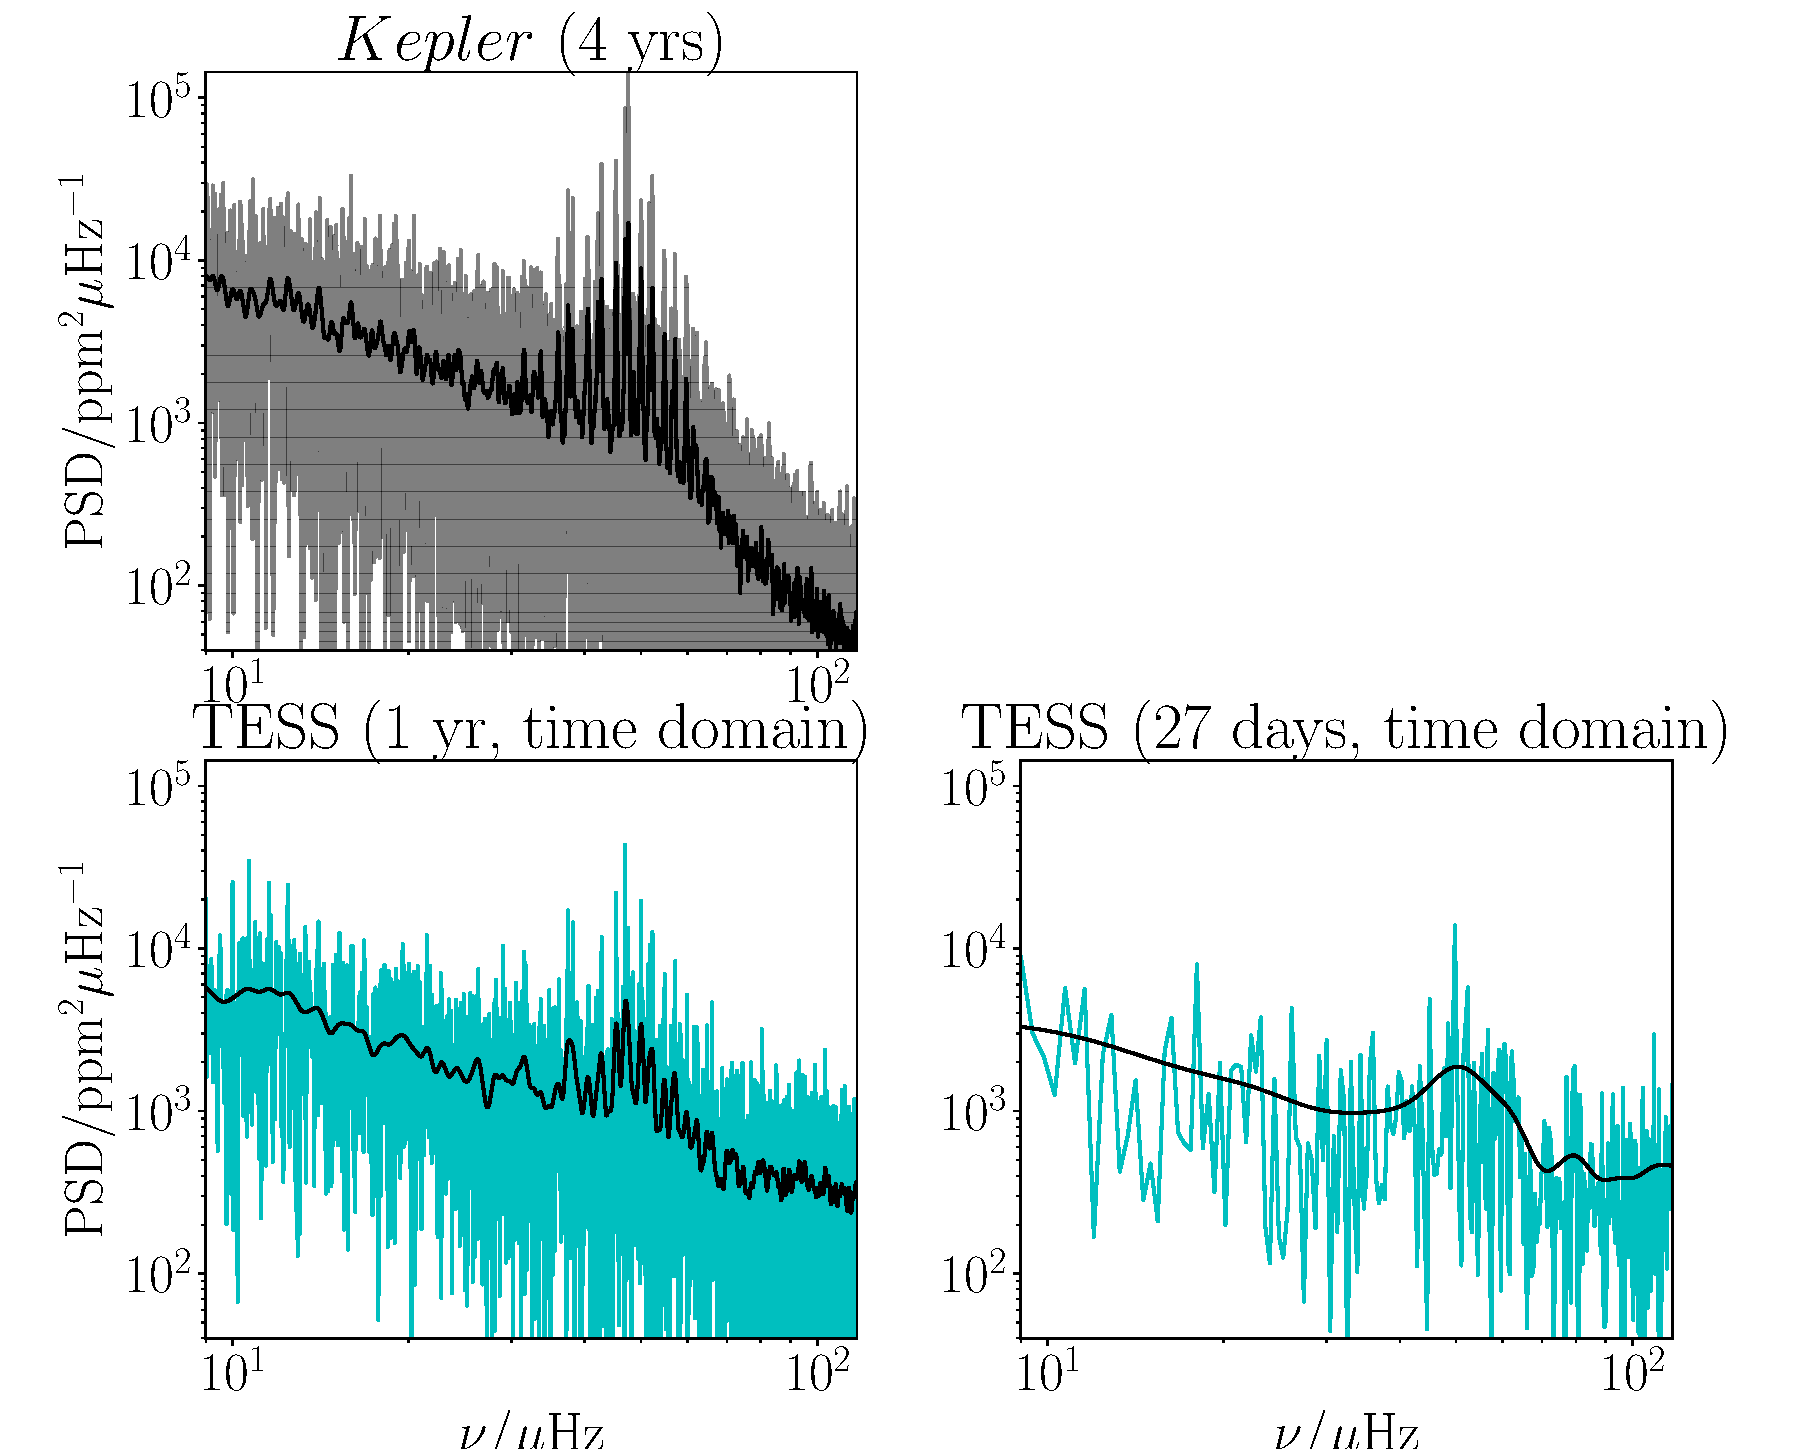
\includegraphics[scale=0.25]{diagnostic_plot3_modes}
	\caption{The Power spectra of KIC 9535399 is plotted three times with moving medians in black. The original Power Spectra is plotted in grey. The power spectra after making the data look like TESS are plotted in blue. The subplot on the bottom left shows 1 year of TESS observation (the maximum). The subplot on the bottom right column shows 27-days (the minimum).}	
	\label{Power Spectra}
\end{figure} 
\begin{figure}
	\centering
	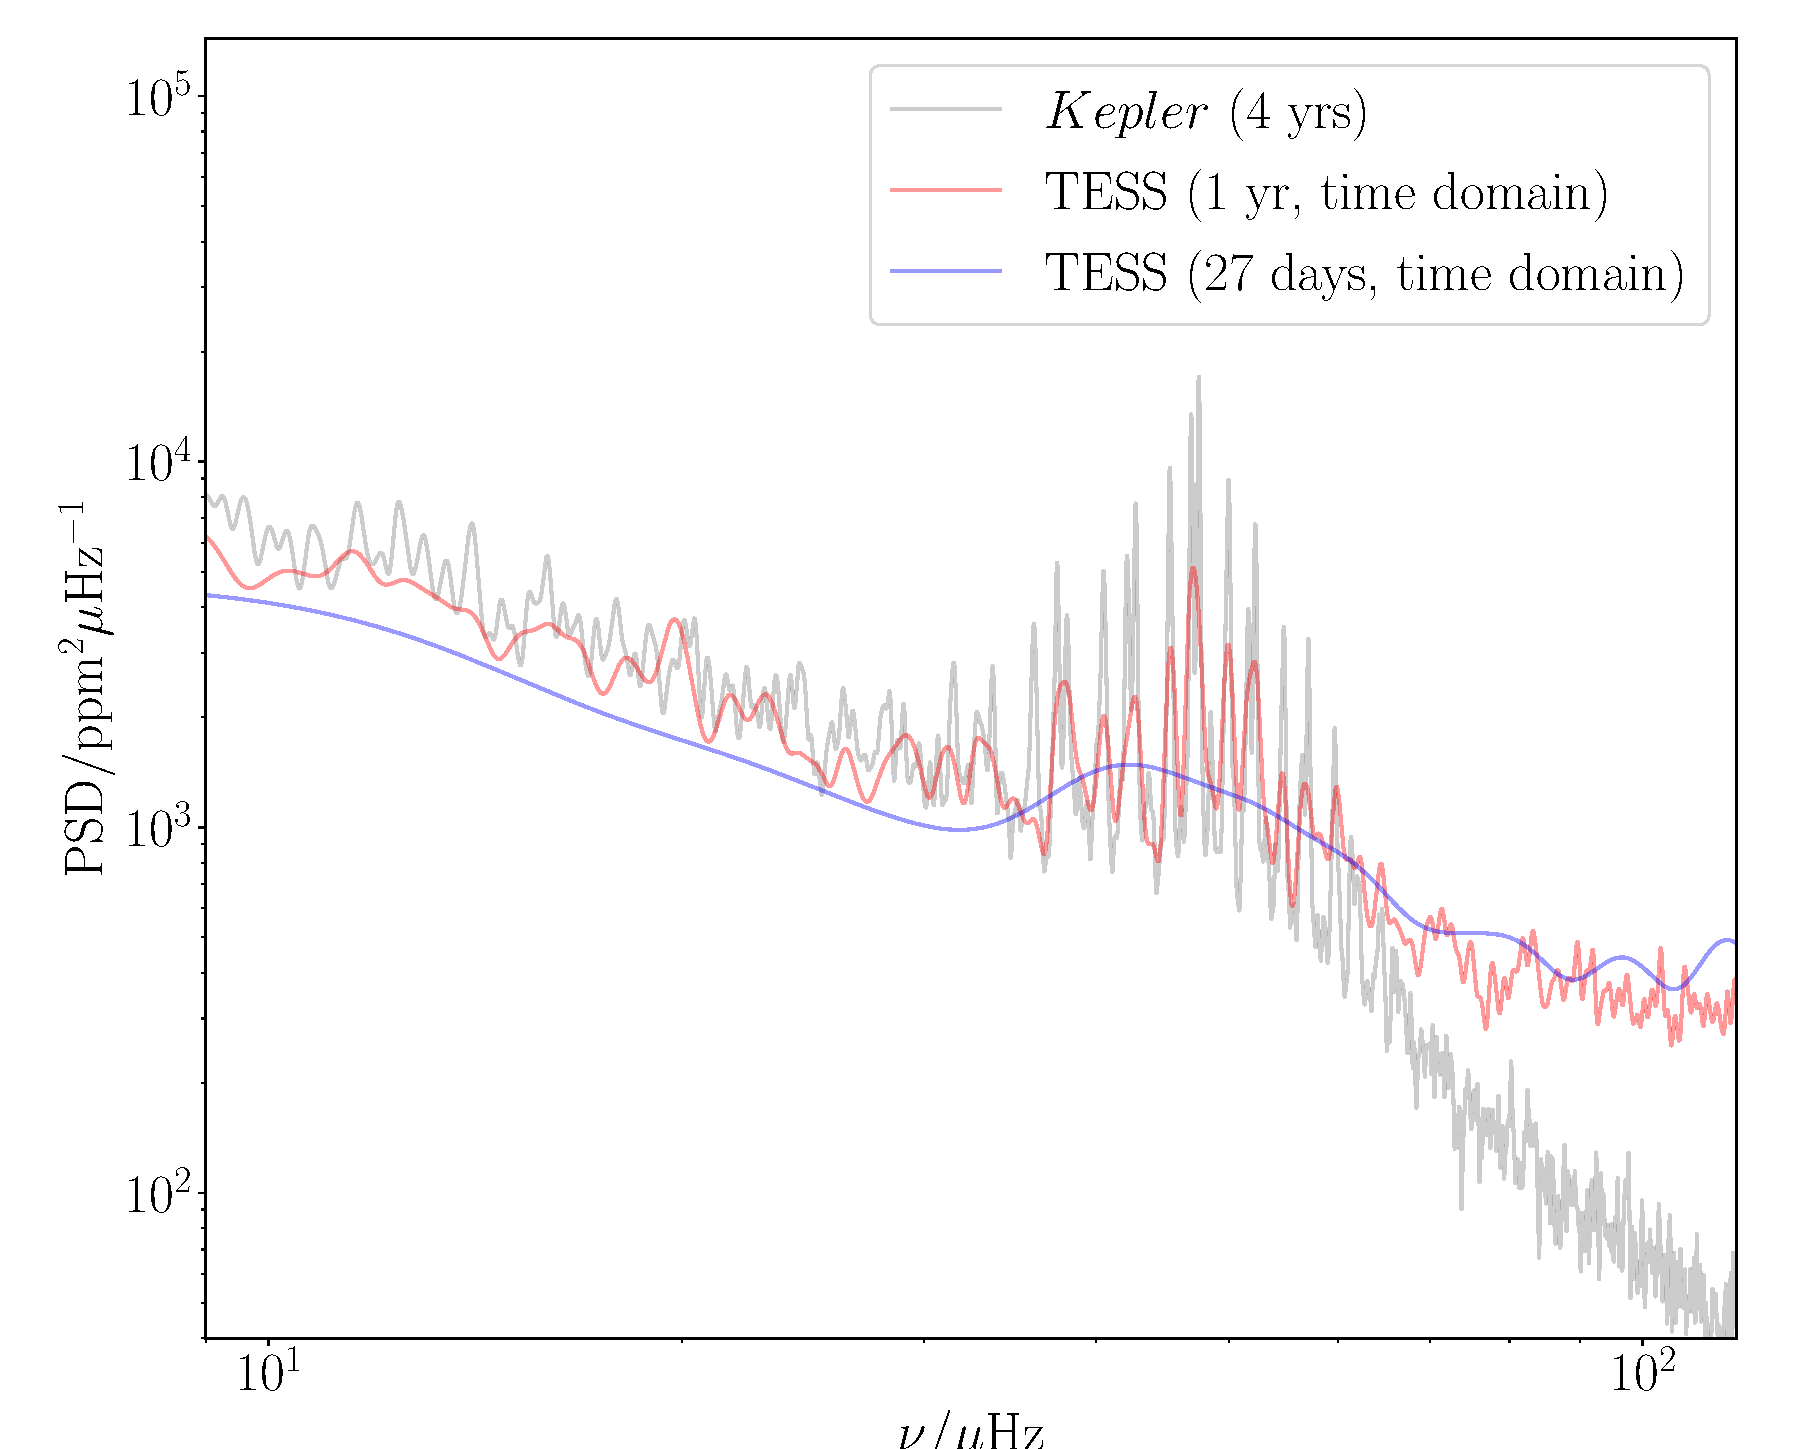
\includegraphics[scale=0.25]{diagnostic_plot4_modes}
	\caption{The Power Spectra of KIC 6768319. The original power spectra is in grey. The data were transformed into 1 year and 27 days of TESS observation. The moving median of these transformations are overplotted.}	
	\label{overplotted PS}
\end{figure} 




\iffalse
\onecolumn
\begin{figure}
	\centering
	\includegraphics[scale=0.5, trim={0 3cm 10cm 0}]{"TRG timeseries flowchart".pdf}
	\caption{Flow chart of the method to convert the data from \kep \ to TESS observations in the time domain.}	
	\label{ts flowchart}
\end{figure} 

\begin{figure}
	\centering
	\includegraphics[scale=0.5, trim={0 3cm 0 0}]{"TRG frequency flowchart".pdf}
	\caption{Flow chart of the method to convert the data from \kep \ to TESS observations in the frequency domain.}	
	\label{fr flowchart}
\end{figure}
\newpage
\twocolumn
\fi


\section{Detection Test}
\label{sect: det_test}

Section \ref{sect: tess-like} described the method to transform the $Kepler$ lightcurves into TESS-like power spectra. A detection test was then run on the stars to determine which modes were detectable by TESS, and which were not.

First, a moving median was used to estimate the underlying background spectrum. The solar-like mode envelope width was used as the frequency range of this moving median. This envelope width was calculated as
\begin{equation}
\Gamma_{\rm env} = 0.66 \: \numax^{0.88},
\end{equation}
from \citet{mosser_characterization_2012}. The moving median provided an estimate of the background $B$ in the power spectrum (ppm$^{2} \mu\rm Hz^{-1}$). This background was divided out of the power $P$ (ppm$^{2} \mu\rm Hz^{-1}$) in the power spectrum to the get Signal-to-Noise ratio of the spectrum,
\begin{equation}
\label{eq:snr}
{\rm SNR} = P/B.
\end{equation}
Once the SNR spectrum for the star was recovered, the SNR values at the mode frequencies were extracted. To ensure the correct SNR values of every mode were used, a window was fitted around each mode frequency from Davies et al. (in prep). The size of the window was given as the linewidth of the mode. The highest value in the window was taken as the SNR of the mode. An example of this for KIC 10587122 is shown in Figure \ref{snr}.
\begin{figure}
	\centering
	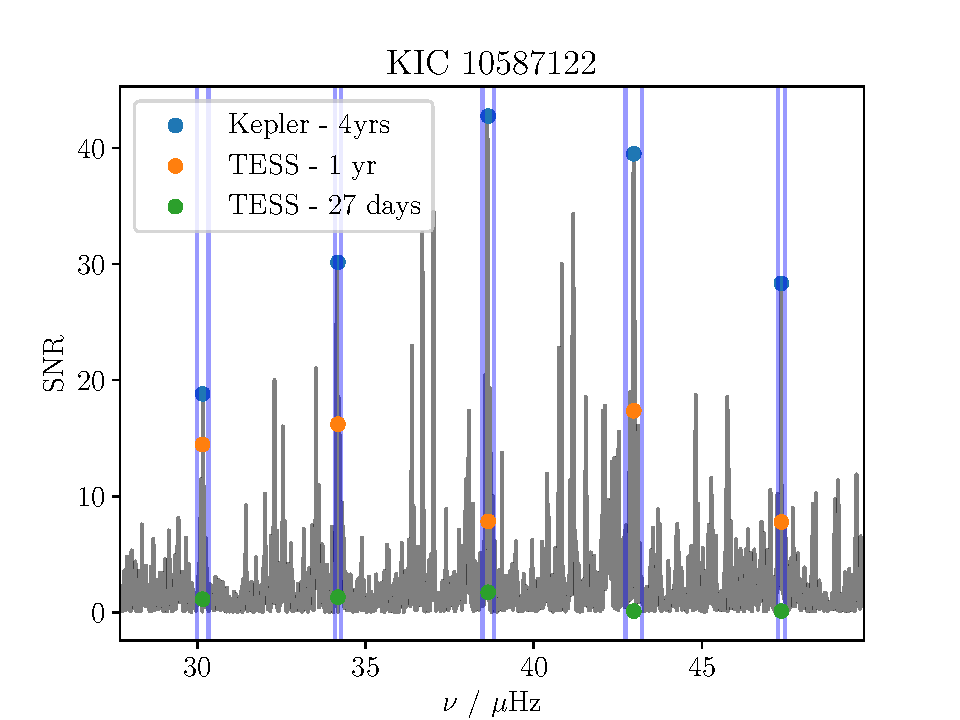
\includegraphics[scale=0.5]{plot4_SNR10587122.pdf}
	\caption{The SNR spectrum of KIC 10587122 after background subtraction. The SNR values of the radial modes in the star were extracted from this spectrum. The highest SNR value within the linewidth of each mode is taken to be the SNR value of that mode. The mode linewidths are shown as blue lines. The values of every mode in the original Kepler spectrum are plotted as blue points. The overplotted orange points are the SNR values after degrading the signal to 1 year of TESS observation. Similarly, the green points are the SNR values of 27 days of TESS observations. The white noise level and reduced observation time severely reduce the SNR of TESS observations compared to \kep.}	
	\label{snr}
\end{figure}

Once all mode SNR values for the star were calculated, a detection test from \citet{chaplin_predicting_2011} was run on each mode. In \citet{chaplin_predicting_2011}, a detection test was used across the entire oscillation envelope. Here, the same detection test was instead applied to individual modes. This method is described below.

The probability $P$ that the SNR value of a solar-like mode of oscillation lies above some threshold ${\rm SNR_{thresh}}$ is
\begin{equation}
\label{eq:pdet}
{P \rm ({ SNR \geq SNR_{thresh}})} =  p .
\end{equation}

A false-alarm probability $p$ of 5\% was set; there is a 95\% chance that the signal is not due to noise. Equation \ref{eq:pdet} is solved for $\rm SNR_{thresh}$ by substituting $P$ with
\begin{equation}
\label{eq:prob}
P = \int_{x}^{\infty} \frac{e^{-x}}{\Gamma(N)} x^{N-1} dx .
\end{equation}
$N$ is the number of frequency bins that the mode occupies. The linewidth of each mode was used as the value of $N$ in equation \ref{eq:prob}.

$\Gamma(N)$ is the Gamma function. The lower bound of Equation \ref{eq:prob} is set to $x=1+{\rm SNR_{thresh}}$. The noise in the $N$ bins is assumed to follow $\chi^{2}$ $2n_{\rm bins}$ d.o.f statistics. 

Once $\rm SNR_{thresh}$ is found, Equation \ref{eq:prob} is solved again. This time it is solved for $P$ by setting $x=(1+{\rm SNR_{thresh}})/(1+{\rm SNR})$. Here, SNR is the observed Signal-to-noise Ratio calculated from Equation \ref{eq:snr}. This calculates the probability that the frequency spike was due to stochastic excitation in the convective envelope of the star.

\begin{figure}
	\centering
	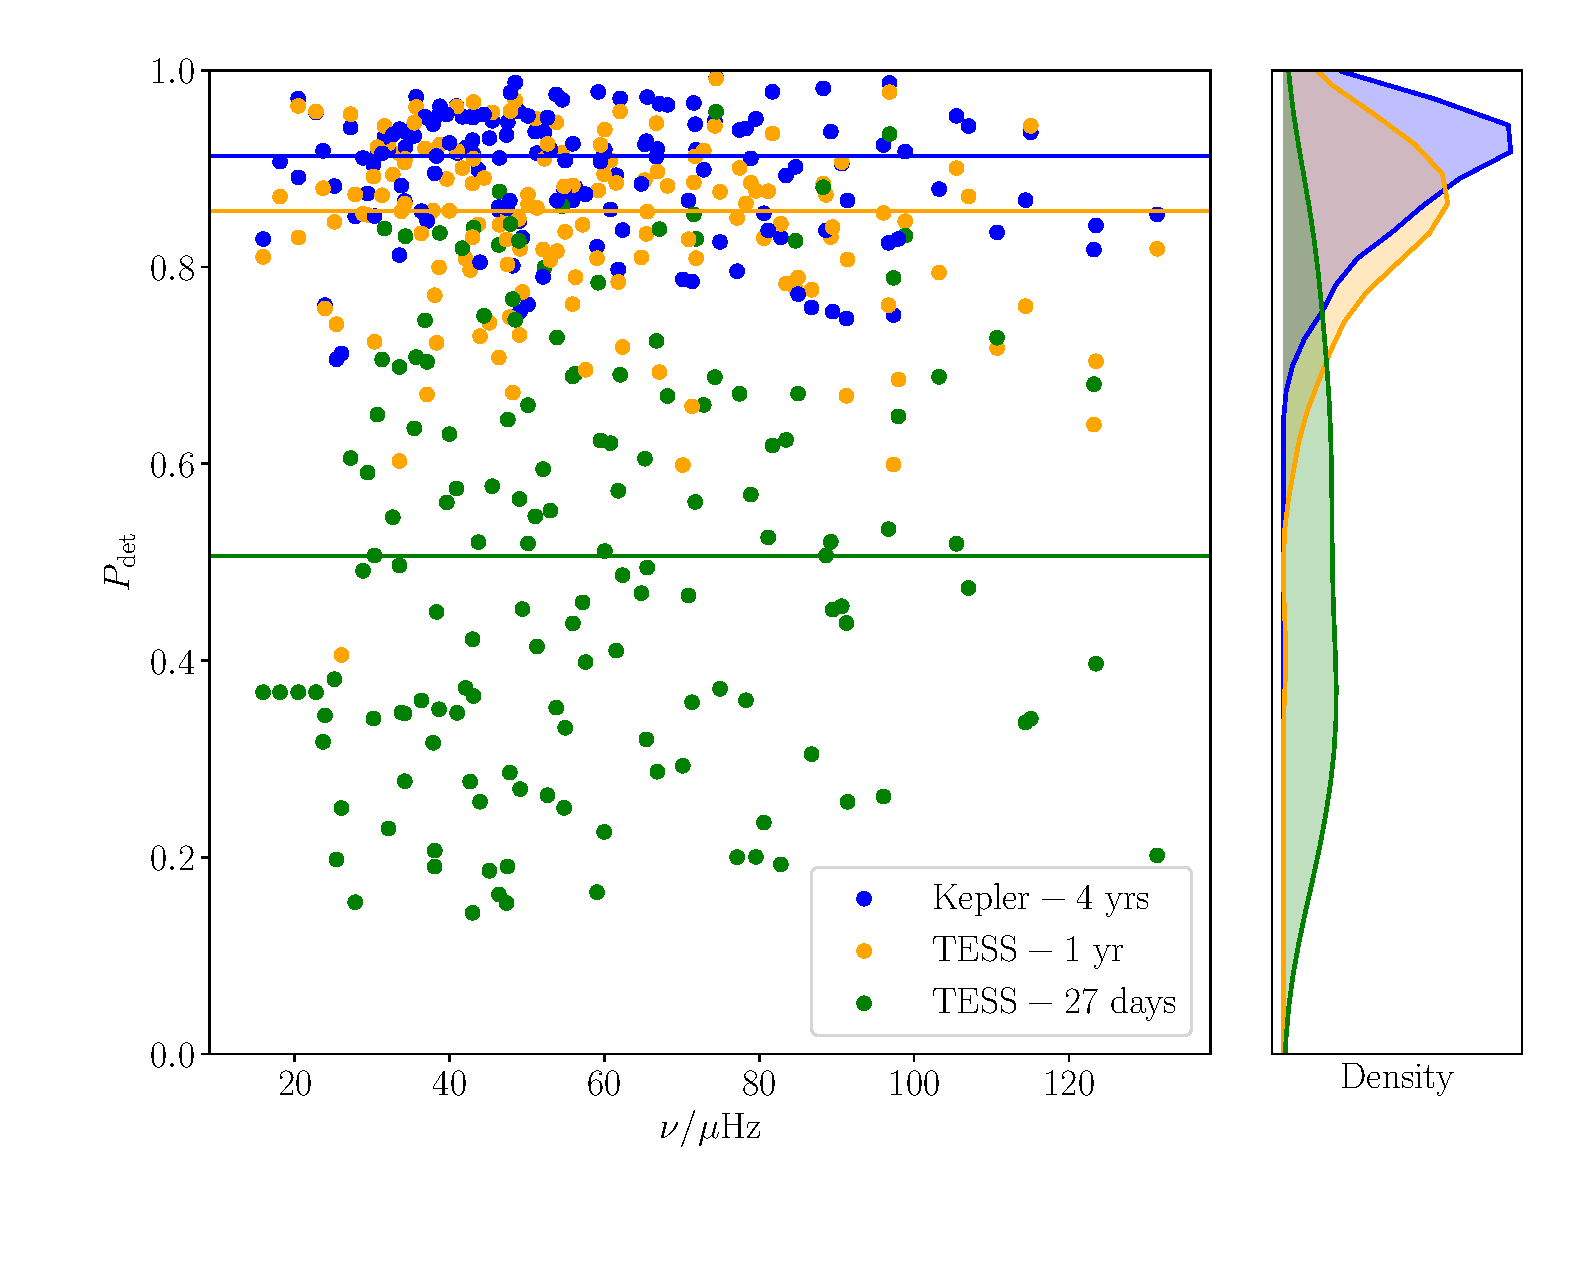
\includegraphics[scale=0.3]{DetTest_Diagnostic_plot3.pdf}
	\caption{A plot showing the result of the detection test, after running on every mode in 20 stars. The results of the original power spectra are plotted in blue. The results of 1 year of TESS observation are in orange. 27 days of TESS observation is in green. At this short an observation, detecting individual modes will be extremely difficult.}	
	\label{fig: modes}
\end{figure}

This detection test was applied to every mode of every star in the sample. Figure \ref{fig: modes} shows the mode detection probabilities from this test for the original \kep dataset, for 1-year of TESS observation and for 27 days of TESS observation. After the \pdet values for the 3 datasets were calculated, a classifier was used to see if these results could be predicted rather than calculated. This is described in Section \ref{sect: classifier}.


\section{Classification}
\label{sect: classifier}

Section \ref{sect: tess-like} describes how the lightcurves of every star were treated before a detection test was run on the oscillations in Section \ref{sect: det_test}. After this, a random forest classifier was used to predict the detection probability of the modes in the Red Giants. 

Classification algorithms work by assessing similarity\footnote{http://www.simafore.com}. In Classification, the training set is separated into groups based on the similarity of the data. The more information that was gained by splitting the data, the better. The data continues to be split until a prediction can be made (in this case about the detection probabilities of 3 radial modes). In decision tree classification, this is done once. 

Here, a random forest classifier was used. This is made up of many independent Decision Trees which have been weighted to predict the detection probabilities of the 3 radial modes. Section \ref{sect: prep} will explain how the data was prepared before the random forest classifier was used.

%It is worth noting that this could be done without using Machine Learning, although it takes much longer. In the age where datasets from missions such as MAST and Gaia \citep{gaia_collaboration_gaia_2016} exist, tools need to be developed to make use of the huge amount of information we now have on stars across the Milky Way. If Machine Learning can replicate the results from a detection test, it could be used as a much faster target selection tool before future observations. It would reduce the computation time needed to generate a list of targets down by orders of magnitude.


\subsection{Preparing the data}
\label{sect: prep}

After removing stars without APOKASC information, 811 stars were left from the original 1000-star dataset. In Section \ref{sect: dataset}, each star had it's \imag value perturbed 100 times. After perturbing the apparent magnitudes, 81,100 stars were available to perform classification upon. This was done 3 times: when the stars were treated as $Kepler$ targets, when they were treated as TESS targets in the Continuous Viewing Zone (1 year of observation), and when the 81,100 stars were treated as TESS targets observed for 27 days. 

Each calculated detection probability from Section \ref{sect: det_test} was then put into a discrete bin (or {\it class}) depending on how likely the mode is to be detected. These discrete classes are given in equation \ref{eq:class}.
\begin{equation}
\label{eq:class}
P_{\rm det} = \left\{ \,
    \begin{IEEEeqnarraybox}[][c]{l?s}
      \IEEEstrut
      2 & if 1.0 $\geq$ \pdet $>$ 0.9  \, , \\
      1 & if 0.9 $\geq$ \pdet $>$ 0.5  \, , \\
      0 & if 0.5 $\geq$ \pdet $>$ 0.0  \, .
      \IEEEstrut
    \end{IEEEeqnarraybox}
\right.
\end{equation}

Using equation \ref{eq:class}, every mode was assigned a discrete class {\texttt [0, 1 or 2]}, depending on how high the probability of detection was for that mode. The same three radial modes ({\it 3 features}) were used for every star: the mode closest to the centre of the power-excess due to solar-like oscillations $\nu_{\rm max; n}$, the radial mode one overtone below that $\nu_{\rm n-1}$, and one overtone above that, $\nu_{\rm n+1}$ [\pdet(1), \pdet(2), \pdet(3)]. It was important to use the same modes for every star so that the algorithm could be trained on the patterns between the variables.

A classifier is an algorithm that can learn a relationship between variables. The classifier will map from some initial information about the star (the X data), to some unknown information (the Y data). In this work, the X data features were magnitude ($K_{p}$ or $I_{\rm mag}$), log($g$), $\pi$, \teff and [M/H]. \logg, \teff and [M/H] values are from \citet{pinsonneault_apokasc_2014}, $\pi$ is from $Gaia$ DR2 \citet{lindegren_gaia_2018} and \imag is from \citet{hog_tycho-2_2000}, with some values imputed using regression (Section \ref{sect: impute}).

The Y data features were the \pdet values of 3 radial modes centred around \numax. An example of the final dataset for 1 year of TESS-like observations are shown in Tables \ref{tab: x dataset} and \ref{tab: y dataset}.


\begin{table}
\begin{center}
\begin{tabular}{|*{7}{c|}}
KIC     & Iteration & log($g$) & $\pi$ & \teff & [M/H] & \imag \\
\hline
9205705	& 1         & 2.758	& 0.688 & 4685 & -0.39 & 9.89  \\
9205705	& 2         & 2.758	& 0.688 & 4685 & -0.39 & 9.19  \\
9205705	& 3         & 2.758	& 0.688 & 4685 & -0.39 & 9.79  \\
9205705	& 4         & 2.758	& 0.688 & 4685 & -0.39 & 11.30 \\
...                                                        \\
9205705	& 100       & 2.758	& 0.688 & 4685 & -0.39 & 7.81  \\
2554924	& 1	        & 2.799	& 0.969 & 4594 &  0.27 & 8.46  \\
2554924	& 2         & 2.799	& 0.969 & 4594 &  0.27 & 9.26  \\
...                                                         \\
\hline
\end{tabular}
\end{center}
\caption{An example of the X-dataset for 1 year of TESS-like observations. Every star has it's magnitude perturbed 100 times. See Table \ref{tab: y dataset} for the equivalent Y-dataset.}
\label{tab: x dataset}
\end{table}

\begin{table}
\begin{center}
\begin{tabular}{|*{5}{c|}}
KIC & Iteration & \pdet(1) & \pdet(2) & \pdet(3) \\
\hline
9205705	& 1     & 1 & 2 & 2 \\
9205705	& 2     & 1 & 2 & 2 \\
9205705	& 3     & 1 & 2 & 2 \\
9205705	& 4     & 1 & 2 & 1 \\
...                         \\
9205705	& 100   & 1 & 2 & 2 \\
2554924	& 1	    & 2 & 2 & 2 \\
2554924	& 2     & 2 & 2 & 2 \\
...                         \\
\hline
\end{tabular}
\end{center}
\caption{An example of the Y-dataset for 1 year of TESS-like observations. Every star has it's magnitude perturbed 100 times. White noise is then added to the timeseries and mode detection probabilities are calculated for 3 radial modes centred around \numax. Lastly, these probabilities are put into discrete classes [0, 1 or 2]. The radial mode closest to \numax is \pdet(2). See Table \ref{tab: x dataset} for the equivalent X-dataset.}
\label{tab: y dataset}
\end{table}



\subsection{Target selection using a classifier}
\label{sect: class-results}

The 81,100 datasets were separated into a training dataset, and a testing set. 70\% of the datasets were used to train the classifier (56,770 stars); 30\% of the stars were used to test the algorithm (24,330 stars). To train the classifier, the X and Y data in the training set was given to the algorithm (X$_{\rm train}$ and Y$_{\rm train}$). Once the classifier had been trained, the X data from the testing set was given to it (X$_{\rm test}$). The classifier then predicted a set of Y data for the testing set (Y$_{\rm pred}$). This was compared to the actual Y data for the testing set (Y$_{\rm test}$). The more similar Y$_{\rm pred}$ is to Y$_{\rm test}$, the better the classifier replicated the data.

Two metrics were used to measure the performance of the algorithm. The first was the precision of the classifier. To calculate the precision, the difference between the 'true' values and the values predicted by the classifier were calculated. This was done for each feature [\pdet(1), \pdet(2), \pdet(3)] separately. The mean of these differences was calculated, and weighted by the number of 'true' values in each feature.

This precision $P_{\rm res}$ is given as
\begin{equation}
P_{\rm res} = t_{\rm p} / (t_{\rm p} + f_{\rm p}), 
\end{equation}
where $t_{\rm p}$ are true-positives and $f_{\rm p}$ are false-positives. The classifier's precision is its ability to not label a negative sample as positive\footnote{http://scikit-learn.org \label{scikit}}.

The second was the Hamming loss$^{\ref{scikit}}$
\citep{wegner_technique_1960} of the algorithm. This was used to give another measure of similarity between the predicted \pdet values Y$_{\rm pred}$, and the testing \pdet values Y$_{\rm test}$;
\begin{equation}
H_{\rm loss}(Y_{\rm test}, Y_{\rm pred}) = \frac{1}{n_{\rm classes}} \sum_{j=0}^{n_{\rm classes}-1} 1(Y_{\rm pred} \neq Y_{\rm test}) \: . 
\end{equation}
A Hamming loss score of 0.0 means that Y$_{\rm pred}$ is identical to Y$_{\rm test}$. A score of 1.0 means that there are no similar values between Y$_{\rm pred}$ and Y$_{\rm test}$. Precision and Hamming loss are similar (but not identical) measures of the success of a classifier. By using both metrics, the usefulness of the classifier can be better assessed. The precision and Hamming loss of the classifier on the \kep and TESS datasets are shown in Table \ref{tab: results}.
\begin{table}
\begin{center}
\begin{tabular}{ |c|c|c|c| }
Satellite & \tobs   & Precision & Hamming loss \\
\hline
\kep      & 4 years & 0.98      & 0.02         \\
TESS      & 1 year  & 0.90      & 0.09         \\
TESS      & 27 days & 0.81      & 0.19         \\
\end{tabular}
\end{center}
\caption{Results of the classifier on the original \kep dataset, and the 1-year and 27-day TESS datasets. The 'Precision' column gives the average weighted precision of the classifier across the 3 classes [0, 1, 2] and 3 features [\pdet(1), \pdet(2), \pdet(3)].}
\label{tab: results}
\end{table}

We also tested the impact of increasing the number of classes in equation \ref{eq:class}, and the range of \pdet values for each class. The number of classes was varied from 2 (i.e the mode was detected (1) or it was not (0)) to 6. The width of each bin was also varied to ensure that bins were not underpopulated. It was found that the 3 classes and \pdet ranges given in equation \ref{eq:class} gave the best predictions for the 3 datasets of 81,100 stars (4 years of $Kepler$ observation, 1 year of TESS observation and 27 days of TESS observation). 

The results for the original \kep dataset and for 1-year of TESS data are very good; the classifier was able to replicate the mode detection predictions of the stars in these cases. This means that a classifier can be used as a tool for target selection for future missions. Once the classifier predicted \pdet values, the stars could be ranked from those with many detected modes, to those with the fewest. In this way, the classifier could be used as the target selection function of solar-like oscillators for TESS. 

For the 27-day TESS dataset, the classifier was able to correctly predict the \pdet values of 81\% of the modes. This is likely to be because with these TESS targets, the dataset is too susceptible to the realization noise of the observation for individual modes to be reliably detected. A mode may be clearly detectable in one 27-day observation, and not another.


\subsection{Feature Importance}
\label{sect: feature importance}

Here, a classifier was used to predict the detection probabilities of individual modes in \kep Red Giant stars. As well as being much faster than a conventional mode detection test, an added bonus of the classifier method is that it returns the 'feature importance' of each label in the X-data.

As Table \ref{tab: x dataset} shows, the X-data features that are given to the classifier are \texttt{[log($g$), $\pi$, \teff, [M/H], \imag]}. Some of these features are more important than others when predicting the detection probability of solar-like modes \texttt{[\pdet(1), \pdet(2), \pdet(3)]}. The relative importance of these columns is known as the feature importance. This feature importance sums to 1.

The feature importances of the X-data columns are given in Figure \ref{fig:feature}. The feature with the highest influence on mode detectability is apparent stellar magnitude \imag. This is not surprising: a higher value of \imag will result in more $\chi^{2}$ 2 Degrees-of-Freedom white noise in the observation. This will make oscillations less likely to be detected above the white noise background.
\begin{figure}
	\centering
	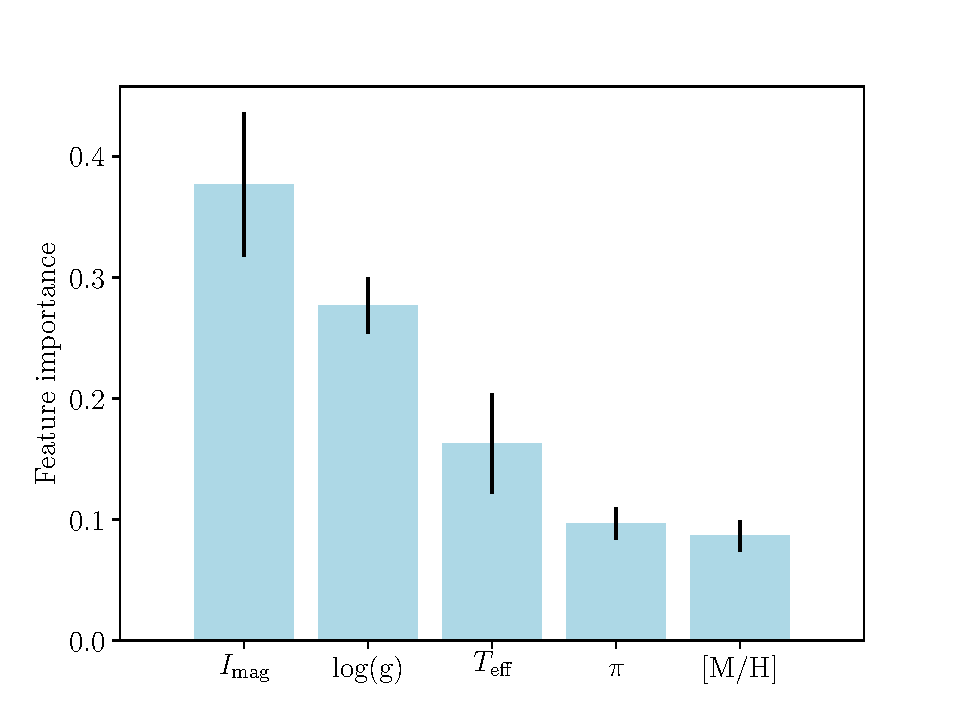
\includegraphics[scale=0.5]{Plot1_featureimportance.pdf}
	\caption{The feature importance of the 5 X-data columns.}	
	\label{fig:feature}
\end{figure}

After the apparent stellar magnitude, surface gravity log($g$) also has a heavy influence on \pdet value. This is because \logg is a proxy for the central frequency of the solar-like mode envelope \numax \:(\numax $\: \propto\logg$). As a star evolves from the Main-Sequence and up the Red Giant Branch, the radius of the star increases. This decreases the \logg and \numax values of the star. \citet{kjeldsen_amplitudes_1995} showed that oscillation amplitude is proportional to bolometric luminosity divided by mass ($A_{\rm osc} \propto L/M$). As a star evolves 'up' the Hertzsprung-Russell diagram, its bolometric luminosity increases while it's mass stays roughly the same. This leads to larger oscillation amplitudes which are more likely to be detected. \citet{mathur_granulation_2011} also gives a good explanation of how the granulation properties (and hence the oscillation profile) change as a star evolves. 

Comparatively, effective temperature \teff is less useful than \logg when predicting detection probability. It is less closely tied to the oscillation properties of the star than \logg, although it is a property used to estimate \numax with the scaling relations \citep{chaplin_predicting_2011}. 

Lastly, parallax $\pi$ and metallicity $\rm [M/H]$ are the least informative features when predicting the detection probabilities of these stars. Parallax is connected to apparent magnitude and \teff, while $\rm [M/H]$ is connected to log($g$). The feature importances of \teff, $\pi$ and $\rm [M/H]$ highlight the additional information that these values bring, as well as indirectly through \imag and \logg.

\iffalse
\begin{table}
\begin{center}
\begin{tabular}{ |c|c| }
Feature      & Feature Importance \\
\hline
log($g$)     & 0.33               \\
$\pi$        & 0.08               \\
\teff        & 0.12               \\
$\rm [M/H]$  & 0.08               \\
\imag        & 0.39               \\
\end{tabular}
\end{center}
\caption{The feature importance of each X-data column. The higher the feature importance, the more important the column was in predicting the detectability of modes inside the Red Giants.}
\label{tab: feature}
\end{table}
\fi

\subsection{Comparing results between different evolutionary states}
\label{sect: evo states}

So far in this paper, the the evolutionary state of the Red Giant population from Davies et al. (in prep) has been ignored when predicting mode detection probability \pdet. In reality, the 1000 \kep Red Giants used in this work are a mixture of Red Giant Branch (RGB), Red Clump (RC) and Secondary Clump (2CL) stars. This Section investigates whether there is any difference in the predictions if the stars are first separated into RGB, RC and 2CL groups. The evolutionary states of the stars in the sample were taken from \citet{elsworth_new_2017}. 

If a Red Giant Branch is massive enough, it will undergo the Helium flash and become a Red Clump star. Red Clump stars are Helium-core burning stars, and all have very similar core masses to each other. These stars have very different $g-$mode period spacings to RGB stars, but are otherwise difficult to differentiate (\citet{chaplin_asteroseismology_2013}, \citet{bedding_solar-like_2011}, \citet{beck_kepler_2011}). If a star is more massive than $\gtrapprox1.8\msol$, it will instead become a Secondary Clump star. This means that it will undergo Helium-core burning without the Helium flash.

The Red Giant dataset was separated into 3 subsets; the RGB, RC and 2CL stars. Each subset was treated in the same way as in Table \ref{tab: results}. Table \ref{tab: evo results} gives the full list of results when the RGB, RC and 2CL stars are separated. 
\begin{table}
\begin{center}
\begin{tabular}{ |c|c|c|c|c| }
Evolution & Satellite & \tobs   & Precision & Hamming loss \\
\hline
RGB       & \kep      & 4 years & 0.98      & 0.03         \\
RGB       & TESS      & 1 year  & 0.83      & 0.16         \\
RGB       & TESS      & 27 days & 0.75      & 0.25         \\
\hline
RC        & \kep      & 4 years & 0.96      & 0.04         \\
RC        & TESS      & 1 year  & 0.90      & 0.09         \\
RC        & TESS      & 27 days & 0.77      & 0.24         \\
\hline
2CL       & \kep      & 4 years & 0.97      & 0.03         \\
2CL       & TESS      & 1 year  & 0.83      & 0.14         \\
2CL       & TESS      & 27 days & 0.69      & 0.30         \\
\end{tabular}
\end{center}
\caption{Results of the classifier when RGB, RC and 2CL stars are separated. Results are shown when the data are treated like \kep stars, and when they are degraded to look like 1-year and 27-day TESS observation. The 'Precision' column gives the average weighted precision of the classifier across the 3 classes [0, 1, 2] and 3 features [\pdet(1), \pdet(2), \pdet(3)].}
\label{tab: evo results}
\end{table}

Table \ref{tab: evo results} shows that there is a negligible difference in predictions between stars undergoing Helium-core burning (RC and 2CL stars) and those that are not (RGB stars). This leads to the conclusion that a classifier can predict the mode detectability of Red Giants at different evolutionary states equally well. It is therefore not necessary to separate out these stars into different evolutionary states before predicting \pdet.


\section{Conclusion}
\label{sect: conc}

The solar-like oscillations of 1000 \kep Red Giant stars from Davies et al. (in prep) were used to determine whether asteroseismic target selection could be done using a classifier. Rather than using Machine Learning to determine the evolutionary state of these stars, a classifier was instead used to predict which individual solar-like oscillations inside the Red Giants could be detected with a future space mission. The mission in question here was TESS, although the same technique can be easily applied to other missions such as PLATO. This tool can also be used to understand target selection bias in previous missions, such as K2 and CoRoT.

%For the first time, Machine Learning was applied to TESS target selection. 1000 peak-bagged \kep Red Giant stars from \citet{davies_asteroseismology_2016} were used to determine whether target selection could be done using a Classifier. 

Firstly, the number of samples was increased by perturbing stellar magnitudes 100 times for each star. These perturbed magnitudes were drawn from a PDF of the noise function (Section \ref{sect: dataset}). After removing stars where global parameters or fitted modes were unavailable, this left 60,000 \kep samples. 

Once the number of samples was increased, the timeseries' were degraded to transform them into TESS-like observations (Section \ref{sect: tess-like}). The dataset length was reduced, white noise was added to the signal, and the bandpass of observation was reddened. A moving median was calculated for the power spectra of these TESS-like Red Giants to estimate the total background in the signal. This was divided out of the spectra, leaving a Signal-to-Noise ratio at every frequency bin (equation \ref{eq:snr}).

A detection test was then run on the SNR values at every mode frequency (Section \ref{sect: det_test}). This gave a detection probability \pdet between 0.0 and 1.0 for every mode. In order to prepare the detection probabilities before Classification, each continuous \pdet value was assigned a discrete class ([0,1 or 2]; equation \ref{eq:class}).

A classifier was then given the global photometric and spectroscopic properties of the Red Giant sample, along with mode detection probabilities for each star. The parameters \texttt{[log($g$), $\pi$, \teff, [M/H], \imag]} from APOKASC \citep{pinsonneault_apokasc_2014}, TGAS \citep{gaia_collaboration_gaia_2016} and $Tycho$-2 \citep{hog_tycho-2_2000} were the 5 X-data features. The \pdet values of 3 radial modes centred around \numax were used as the Y-data features. % see http://scikit-learn.org/stable/modules/multiclass.html
The classifier used the global stellar parameters (the X-data) to make predictions about mode detectability (the Y-data). The stars with the largest number of detected modes could then be selected as the Red Giants for observation by TESS. 

The classifier successfully made predictions about the original 4 years of Kepler data; the algorithm had a weighted precision 0.98 across the 3 \pdet features. This confirms the proof of concept that classifiers can be used as a way to select solar-like asteroseismic targets before future missions. As well as this, this shows that it can be used to investigate any possible target selection bias, for example in K2 or CoRoT. Classification vastly reduces the computation time required to produce a target selection function, especially when large datasets are involved ($\geq50,000$ stars).  

Degrading the Red Giant data to make predictions for 1 year of TESS observations was also successful. The predicted mode detections scored a weighted precision of 0.90 across the 3 \pdet features. This illustrates that Classification is a valid target selection method for TESS targets in the Continuous Viewing Zone (CVZ, \citep{ricker_transiting_2014}).

Using the classifier on 27 days of TESS data returned detection predictions with a precision of 0.81. This is too low for the classifier to be used to select solar-like oscillators for 27 days of TESS observation. The precision is lower when stars are observed by TESS for 27 days because the white noise level is too high and the length of observation is too short to make robust predictions of individual solar-like oscillations. It may be that individual solar-like oscillations cannot be detected in 27 days of TESS data. If this is the case, then the classifier should not be expected to make robust detection predictions for these stars.

%It is important to note that there are two sources of noise to consider with this \kep dataset. white noise from equations \ref{eq:kep noise} and \ref{eq:tess noise} and stellar granulation noise. Each star in the dataset has one timeseries with one set of fitted modes available. One realisation of the star. This gives only one value of the stellar shot noise. This is not an issue with 4 years fo Kepler data (where modes are easily detectable). It is also not an issue for 27 days of TESS, when white noise has a much bigger impact on mode detectability. In order to test if this is a significant factor for 1 year of TESS data...

%Used multilabel multiClass classifier: 3 Pdet labels for every star, several possible classes: (0,1 or 2). Hamming loss gives score of.... Lower hamming loss score, the better. minimum score=0 (best), maximum score=1 (worst). It is the fraction of labels that are incorrectly labelled. % see https://stackoverflow.com/questions/38697982/python-scikit-learn-multi-class-multi-label-performance-metrics




\bibliographystyle{mnras}
\bibliography{TRG}

\bsp
\label{lastpage}
\end{document}
